\documentclass[11pt]{article}
\usepackage{amsmath, amssymb, amsthm, amsfonts,cite,alltt,clrscode}
\usepackage[english]{babel}
\usepackage{graphicx}
\usepackage{caption}
\usepackage{wrapfig}
\usepackage[list=true,listformat=simple]{subcaption}
\usepackage{hyperref}
\renewcommand{\tt}{\texttt}
\newtheorem{theorem}{Theorem}[section]
\newtheorem{lemma}[theorem]{Lemma}
\newtheorem{proposition}[theorem]{Proposition}
\newtheorem{corollary}[theorem]{Corollary}
\newenvironment{definition}[1][Definition]{\begin{trivlist}
\item[\hskip \labelsep {\bfseries #1}]}{\end{trivlist}}
\newenvironment{example}[1][Example]{\begin{trivlist}
\item[\hskip \labelsep {\bfseries #1}]}{\end{trivlist}}
\newenvironment{remark}[1][Remark]{\begin{trivlist}
\item[\hskip \labelsep {\bfseries #1}]}{\end{trivlist}}
% Complex \xxx for making notes of things to do. Use \xxx{...} for general
% notes, and \xxx[who]{...} if you want to blame someone in particular.
% Puts text in brackets and in bold font, and normally adds a marginpar
% with the text ``xxx'' so that it is easy to find. On the other hand, if
% the comment is in a minipage, figure, or caption, the xxx goes in the text,
% because marginpars are not possible in these situations.
{\makeatletter
\gdef\xxxmark{%
\expandafter\ifx\csname @mpargs\endcsname\relax % in minipage?
\expandafter\ifx\csname @captype\endcsname\relax % in figure/caption?
\marginpar{xxx}% not in a caption or minipage, can use marginpar
\else
xxx % notice trailing space
\fi
\else
xxx % notice trailing space
\fi}
\gdef\xxx{\@ifnextchar[\xxx@lab\xxx@nolab}
\long\gdef\xxx@lab[#1]#2{\textbf{[\xxxmark #2 ---{\sc #1}]}}
\long\gdef\xxx@nolab#1{\textbf{[\xxxmark #1]}}
% This turns them off:
% \long\gdef\xxx@lab[#1]#2{}\long\gdef\xxx@nolab#1{}%
}
\setlength{\parindent}{0.0in}
\setlength{\parskip}{0.1in}
\usepackage[margin=1in]{geometry}
\begin{document}
\title{MITTunnels: A WiFi based localization system for mobile devices}
\author{Andrey Kolchanov\thanks{Skoltech, \protect\url{andrey.kolchanov@skoltech.ru}}, Jayson Lynch \thanks{MIT Computer Science and Artificial Intelligence Laboratory,
32 Vassar Street, Cambridge, MA 02139, USA,
\protect\url{{mpersu,jaysonl}@mit.edu}}
, Madalina Persu\footnotemark[2]}
\date{\today}
\maketitle
%\tableofcontents
%\pagebreak
%
%\listoffigures
%\pagebreak
%
%\listoftables
%\pagebreak
\section{Introduction}
This project implements a WiFi-based indoor positioning system for navigating the MIT Tunnels without GPS. Localization is done based on the WiFi adapters that are visible to an Android device. Notably this solution doesn’t require any additional hardware from the user besides an Android phone and can be deployed without any changes to the AP’s in a region or knowledge of their specific location.

\section{Technical Problem}
Many of the buildings at MIT are connected through an extensive network of underground tunnels. A significant proportion of the student body uses them every day, especially during winter time, since they provide an easy transportation alternative to facing the cold weather outside. One major drawback from using the tunnels is that since they are located underground, there are very few reference points to orient oneself and moreover, most of the tunnels look alike. From a practical perspective, our project addresses this problem by providing a user friendly navigation tool.
From a technical point of view we are faced with the problem of indoor localization. GPS is the default means used to perform accurate outdoor localization. However, GPS signals are carried through waves at a frequency that does not move easily through solid objects. Applications that use GPS to get the user’s location don't work properly in many indoor environments. For the particular scenario we are considering, since the MIT Tunnels are located underground, there is little to no GPS signal. In addition, GPS is currently not designed to give accurate height locations, which makes it unsuitable for detecting which floor in a building a user is on. Given all these considerations, GPS is not a suitable means of achieving indoor localization, hence we have to look for a different approach.

\section{Previous Work}
There has been a large body of work on wifi based localization methods; however, when we look at solutions that can be deployed purely in software on the user side, the body of work is cut down significantly. Two primary methods that fall into this category are Wifi based RSSI and Wifi fingerprinting.

RSSI methods are based on the idea that the signal strength of a wireless AP will attenuate as one moves farther away. In an ideal setting, we know the strength falls off as the distance squared. Thus we could calculate the distances to multiple AP's with known locations and intersect those spheres to find the current device location. However, this methods becomes complicated by multi-path effects, and different attenuation rates through different mediums. Yongguang Chen and Hisashi Kobayashi show the feasibility of this method and discuss various models and controllable parameters to help deal with these added difficulties.\cite{RSSI1} This method does require knowing the position of the AP's so it doesn't yet fit our criteria; however, Chintalapudi, Lyer, and Padmanabhan show how we can use machine learning techniques to infer the location of the APs using this technique, especially if assisted by a small number of GPS readings.\cite{RSSI2}

To avoid some of these complications we went with a Wifi fingerprinting method. An early study of this technique was done using RFID by Bahl and Padmanabhan. The technique exploits the fact that as long as the environment is the same, the signals should be the same in the same locations. \cite{RFID} This sidesteps multi-path problems, and later fingerprinting methods using Angle of Arrival detection actually benefit from the multi-path signal. A 2012 paper does investigate Wifi fingerprinting as a localization method, but concludes accuracy below 6-8m is not possible. The main focus of their paper is on inter-phone range finding, localizing between phones, and synthesizing their measurements. \cite{Push2012} Despite this technique being an easy to deploy candidate there does not seem to be significant literature or research on it's capabilities and techniques to improve the results.

There is also significant corporate interest in wifi based localization techniques; however, the majority of this work is not publicly accessible and thus cannot be read or improved upon by outside researchers. In 2011 Google launched an initiative to provide indoor maps and localization to mobile phone users. They claim 5-10m of accuracy, however, there are no details about their methods.\cite{CNNGoogle} We also see companies like Skyhook which claim to use a synthesis of GPS, cell-based, and wifi localization.\cite{Skyhook} Finally, Microsoft has started holding an annual contest to perform indoor localization.\cite{Microsoft} A number of the 2014 competitors describe using Wifi fingerprinting or sensor synthesis methods; however, even here the details of the project and techniques are missing.

Another indoor localization approach that uses extra hardware is iBeacon, which relies on Bluetooth beacons. The technology enables a smartphone or other device to perform actions when in close proximity to an iBeacon. iBeacon uses Bluetooth low energy proximity sensing to transmit a universally unique identifier picked up by a compatible app or operating system. The identifier can then be looked up over the internet to determine the device's physical location or trigger an action on the device such as a check-in on social media or a push notification.

Various vendors have made hardware iBeacons that come in a variety of form factors, including small coin cell devices, USB sticks, and generic Bluetooth 4.0 capable USB dongles.\cite{iBeacons}

\section{Solution}
Our proposed solution is to do indoor localization based on the MAC addresses of the different WiFi access points within range of a mobile device at a given location. To this end we created an application for Android platform that enabled us to acquire a database of physical points and the associated MAC addresses and their signal strengths. We used the data we collected to train a localization algorithm which when queried with a list of MAC addresses, outputs an estimation for the physical location where those might have been seen. We finally created a user friendly version of the app that displays the computed estimation on a map of the MIT tunnels, as can be seen below. The application is available in Google Play using the following link: \url{https://play.google.com/store/apps/details?id=com.mit.mitlocator} for Android 2.2 and higher.
\begin{figure}[h]
\centering
\begin{subfigure}[b]{0.45\textwidth}
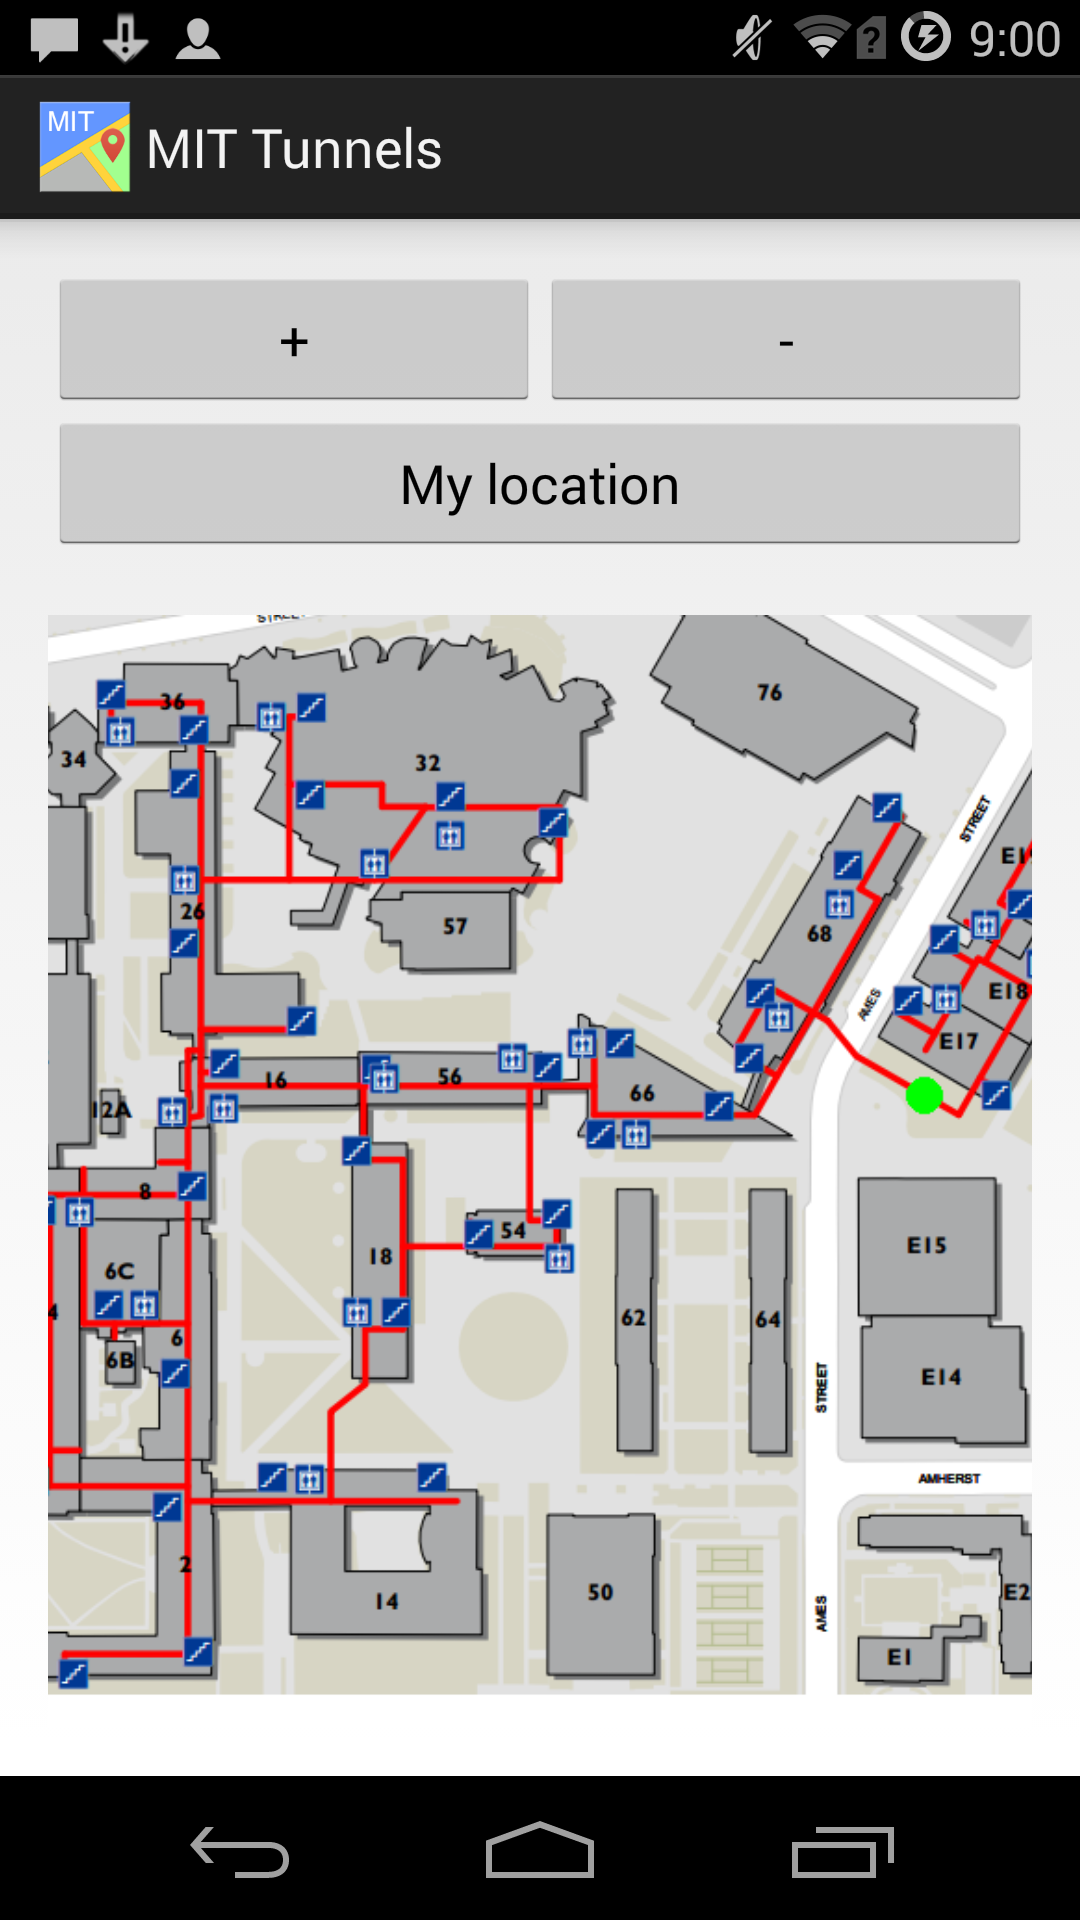
\includegraphics[width=\textwidth]{ScreenshotTunnels1}
\label{fig:app1}
\end{subfigure}%
\qquad \quad
%add desired spacing between images, e. g. ~, \quad, \qquad, \hfill etc.
%(or a blank line to force the subfigure onto a new line)
\begin{subfigure}[b]{0.45\textwidth}
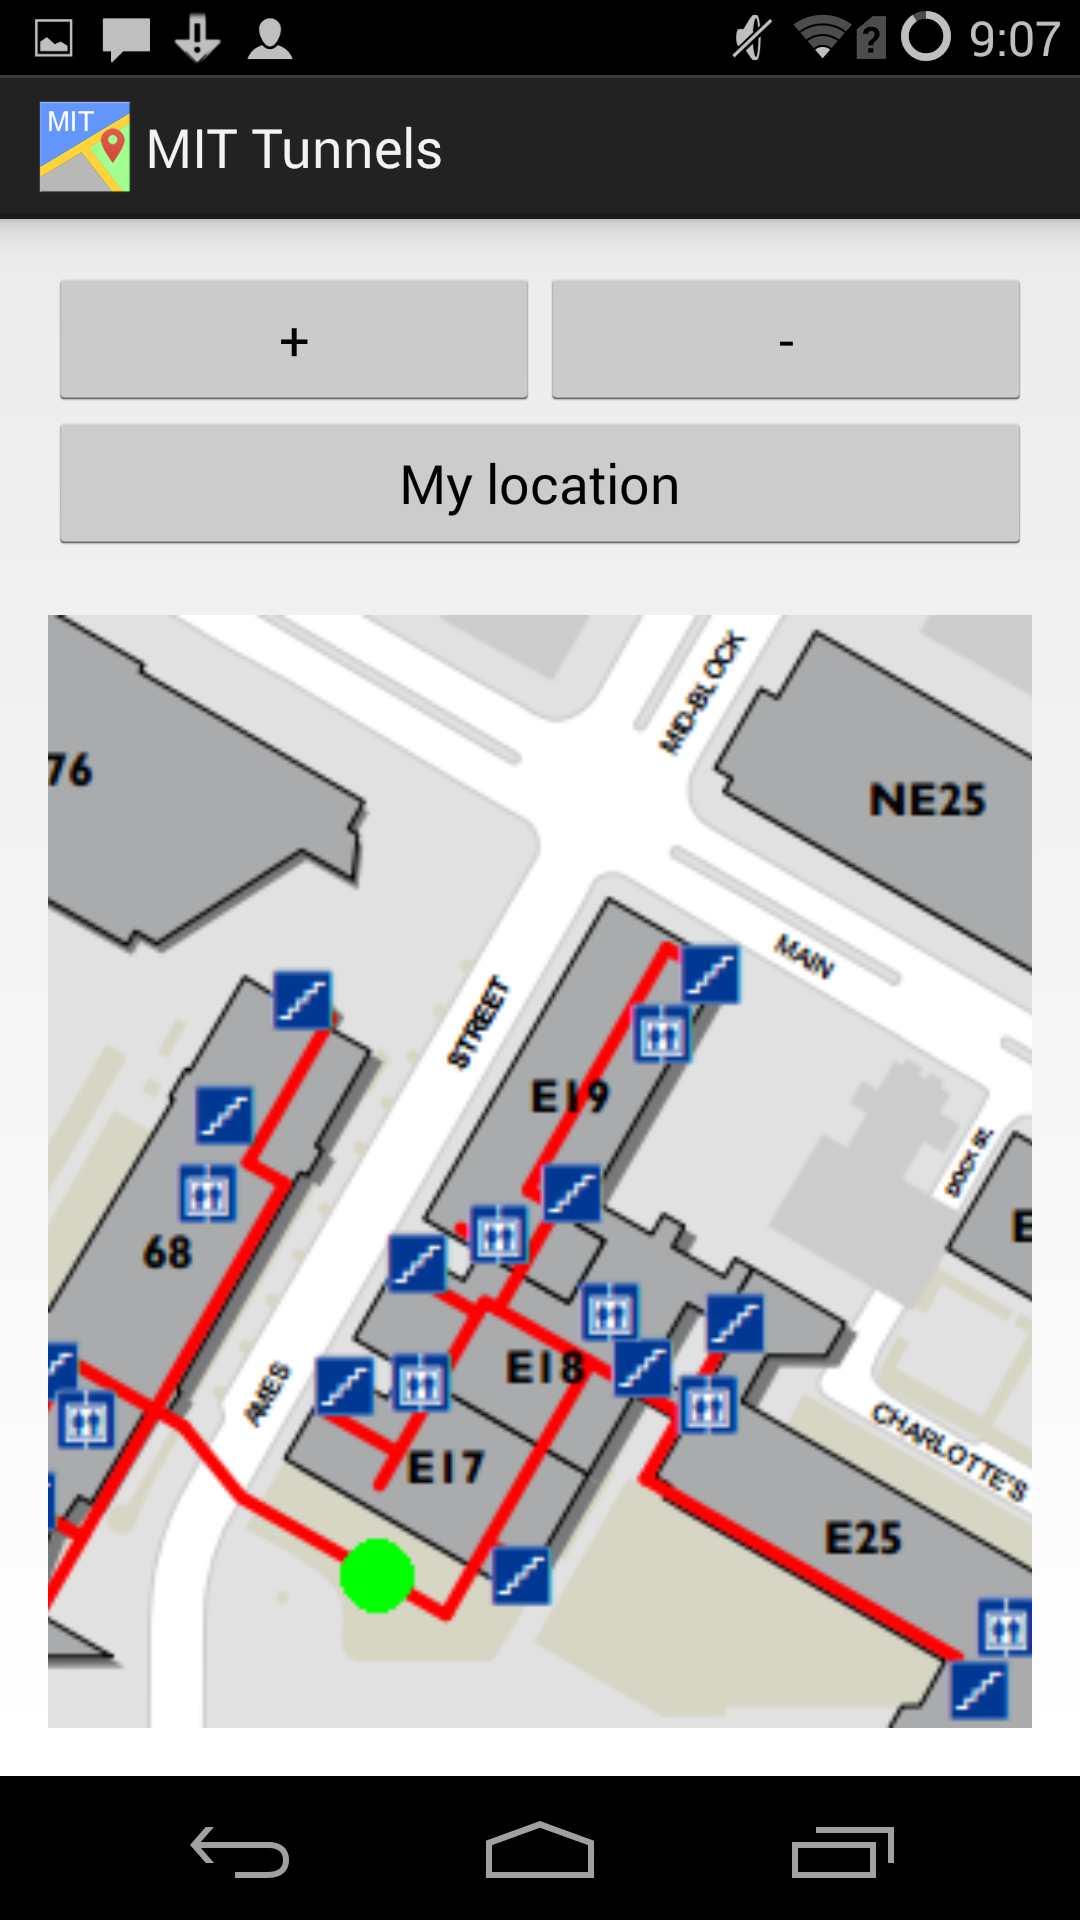
\includegraphics[width=\textwidth]{ScreenshotTunnels2}
\label{fig:app2}
\end{subfigure}
\caption{Figures 1 and 2. Application screens with determined position of the device on the map of MIT Tunnels}
\end{figure}
We expand on each of the components of our solution in the following subsections.
\subsection{Application Requirements}
\subsubsection{Use cases}

Use case 1. User runs the application\\
On this use case, the app should load a dataset. There are two ways to complete it: load data from an internal storage or from a server. For the end-user application that is available in Google Play we chose the first option since it enables the application to work even if the user is using a device that doesn’t currently connect to the Internet. For the developer application that allows to collect data for saving them into a database, we chose the second option.

Use case 2. User presses My location button\\
On this use case, the application scans all available WiFi access points in a visible range and applies the algorithm to find a most likely physical location from saved locations in the database.

Use case 3. User interact with a map\\
In the application we created a map engine that allows to work with any physical map (in png or svg formats) and associates a list of scanned wireless access points with the points on the map.

\subsubsection{Application screens}
Currently the application has only one screen with the map and navigation controls. It provides easy and comfort way to interact with the app. In the future the app will have a Navigation screen to choose a destination and show routes to the location of the destination.

\subsection{Application Design}
We have chosen Android as a platform for our solution since Android provides access to WiFi state on a mobile device. It allows us to scan all available WiFi access points on a certain location and make a suggestion about where its user may be. Other popular mobile platforms, such as iOS and Windows Phone, don’t provide access to the network state. Particularly on iOS, you can get info only about the current WiFi network that the user is connected to. Because of these considerations it is impossible to deploy our solution on those mobile platforms.\\

We implemented the solution for Android 4.1 Jelly Bean with API level 16 on Eclipse IDE. The source code of the application is available on the GitHub repository \\
\url{https://github.com/andrey4623/MITtunnels}. 
The minimum Android version that the application supports is 2.2.

The application logic has the following functions:\\
for working on data:
\begin{itemize}
\item loadDataFromDatabase() - loads dataset from an internal storage;
\item getLocation() - determines a current physical location;
\item getDeviceName() - returns a device name (WiFi adaptors on different devices may be different);
\end{itemize}
for working on a map:
\begin{itemize}
\item checkBorders() - checks does map came out of borders;
\item zoomIn() - zoom a map in;
\item zoomOut() - zoom a map out;
\item onSwipeRight() - moves a map right;
\item onSwipeLeft() - moves a map left;
\item onSwipeTop() - moves a map top;
\item onSwipeBottom() - moves a map bottom;
\item drawMap() - repaint a map on a device screen;
\item loadMap() - loads graphic map from an internal storage.
\end{itemize}

for working on a network:
\begin{itemize}
\item isNetworkAvailable() - returns where is network available or not.
\end{itemize} 

\begin{figure}[h]
\begin{center}
	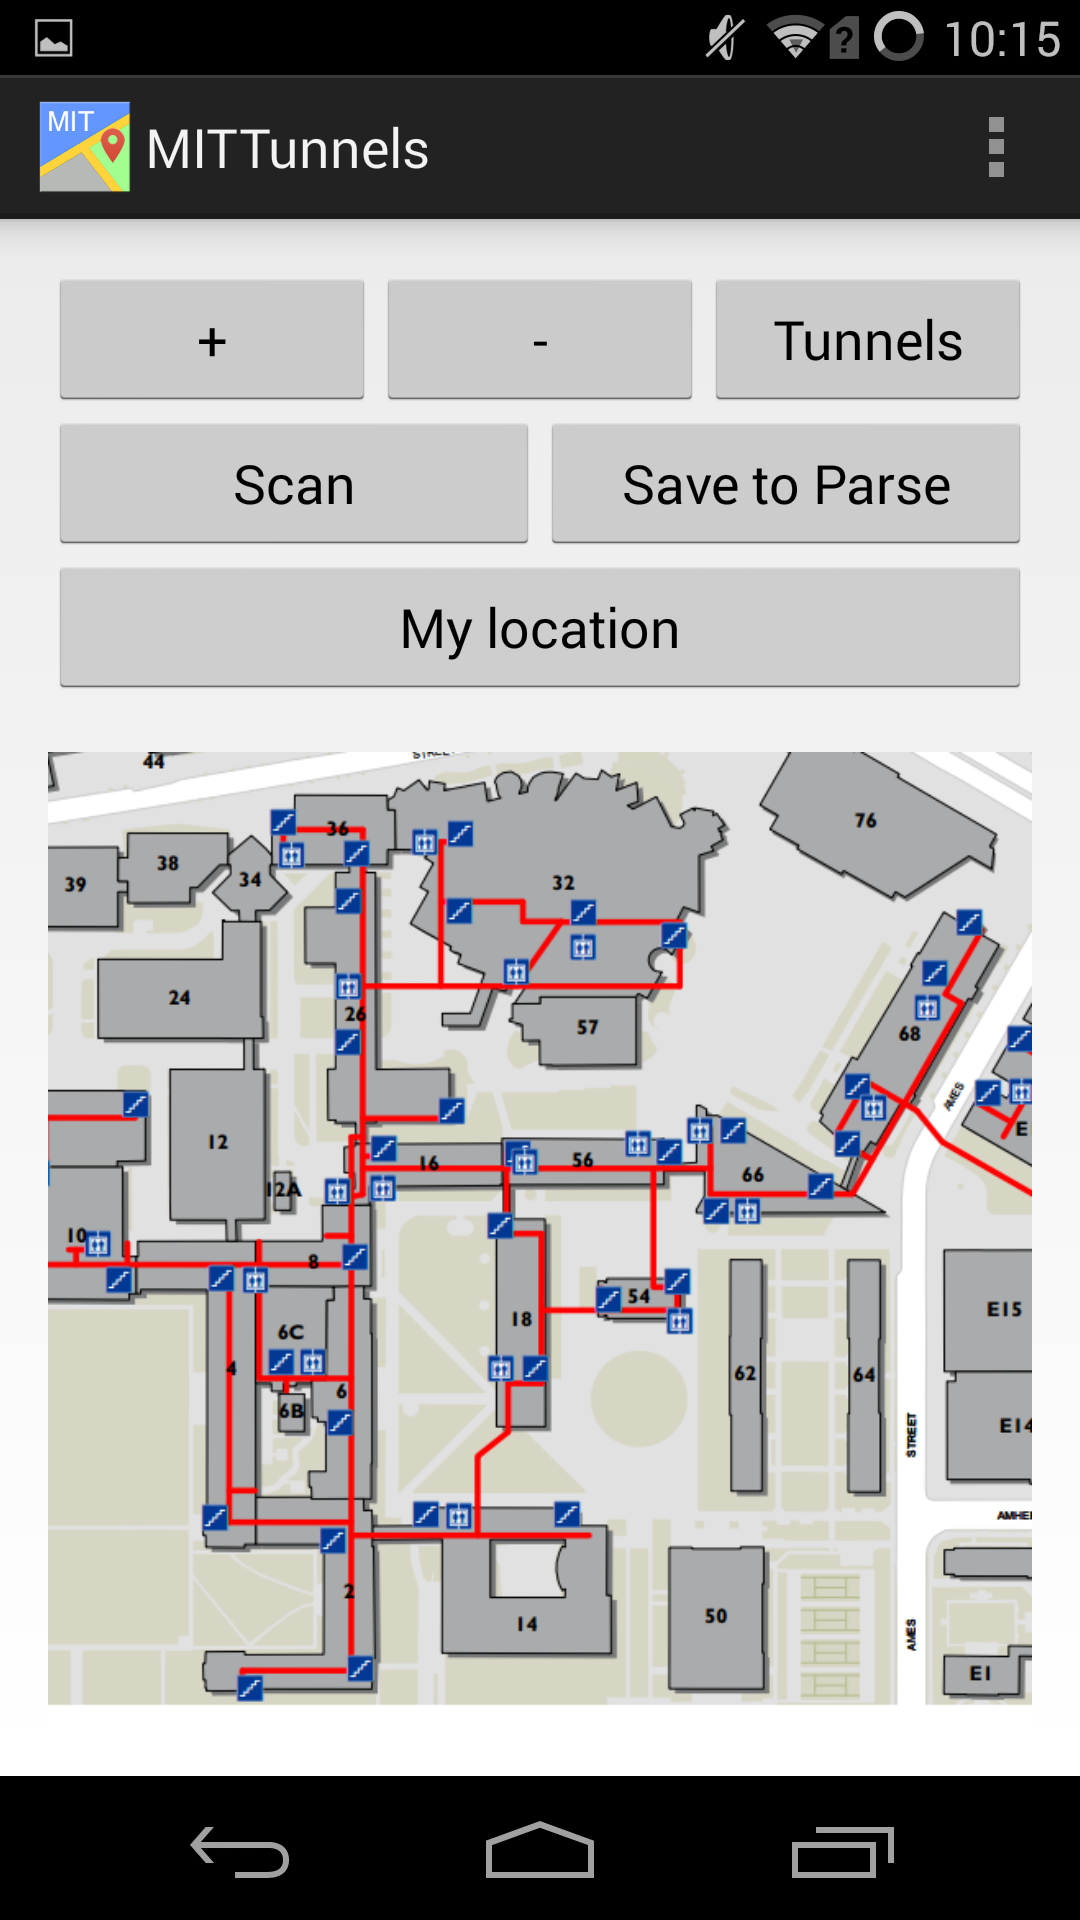
\includegraphics[width=0.45\textwidth]{ScreenshotDeveloper.png}
\end{center}
\caption{Screenshot of a service application}
\label{fig:tunnels_all}
\end{figure}

We also have a modified version of the application that enables the user to collect data for the database. This version has as additional functions ‘Scan access points’ and ‘Save data to the database’.

We chose Parse (\url{https://parse.com/}) as a cloud platform for storing data. Each time an administrator saves scanned data, the app saves them into Parse. The administrator can choose a correct version of data and put them into a public app.\\

Our solution can be applied to other buildings, office spaces, warehouses, etc. The process of creating a map is quite easy: the administrator should go throw all routes in a building and scan WiFi access points into the app. Then the data file should be placed in the folder of the public app and the public app should be compiled.
\subsection{Algorithm}
In this section we present the algorithm we currently have in the most recent version of the application. For the purpose of experiments we used the data in Python and tried different algorithms. We noticed a different one works better, even though it takes more time to run, and we plan to update it. More details about the algorithms used with the Python code can be found in the Experiments section. The Python script source code can be found in the GitHub repository as well.
Let $Macs(x)$ be a list of all MAC addresses visible at a particular point $x$. Let $D$ be our database of points, the training set. Each element of $D$ contains a physical location $x,y$ together with a MAC address within range of $(x,y)$. Subsequently, the dataset is transformed such that each element contains a physical location $(x,y)$ together with a list of MAC addresses within range of $(x,y)$. To output a guess for a position $(x,y)$ on input $Macs(x,y)$ the localization algorithm goes through $D$ and computes the minimum signal distance in the space of $Mac$ addresses between the input and any point in the database. The output is the average of the $(x,y)$ coordinates of all points in the database $D$ found at this minimum distance.
\section{Problems encountered and how they were addressed}
\subsection{Orientation Bias}
While collecting data in the initial stages of our project, we noticed that the number of APs in range and their signal strength change with the phone orientation even when the physical location is unchanged. Some intuition behind why this phenomena might appear is that antennas are directional, they cannot pick up signals parallel to the body of the antenna and thus changing their orientation may change the received signals. Another explanation might be that the body of the person holding a phone is a strong enough obstacle that is significantly changes the signal signal when position between android device and AP, potentially completely blocking weak signals.

To mitigate this issue we modified the application to collect data 5 times at each point. While collecting the data we rotated the phone so we can collect from multiple orientations. The data was subsequently averaged at each point before being used for localization. Taking an average in this manner means the result will be farther away from any particular reading the user will likely take, but hopefully makes up for it by being reasonably close to any of them. For the signal distance, we are essentially shrinking all of the signals seen at each orientation, and for the MAC address seen, the averaging basically amounts to taking the union of all of the APs seen. It’s quite possible that the changes are significant enough that we don’t want to average the readings, but instead should take readings at many different orientations and match onto those specific fingerprints. Further testing and analysis of the impact of phone and user orientation are needed to determine the most effective solution to this challenge.\\

\subsection{Different Devices}
We noticed that signal strength at given locations is not consistent across devices. This made sense given that devices differ in terms of hardware used, hence the performance of their WiFi antennas would be different too. One potential idea to go around this issue would be to try and calibrate the signal strength based on the type/generation of the device you’re using. A more indepth study of the differences in signals picked up by various devices would be needed to perform this sort of correction. Another idea would be to gather datasets for each significantly different category of device. This generally seems infeasible to scale and update, but may be a solution for certain use cases. Given the available time we decided to not use signal strength as a measure of distance but rather 0-1 distance, by only taking into account if you see a specific AP or not. While losing some potential useful information, this measure proved to be more reliable across devices. The Experiments section has a more detailed description of our preliminary study of different devices.

\subsection{Changing Environment}
Changing the environment in a location may change the signals received at that location. Since this changes the signal at a given location this could potentially be a huge problem for localization. We investigated some of these effects around G5, though luckily the MIT tunnels don’t seem to vary in a very significant manner. There are three categories of changes we’ve identified which have different potential solutions. We will call these short term changes, long term changes, and periodic changes.\\
Short term changes are changes that occur at unspecified times and may be altered multiple times a day. For example, one significant change we encountered is whether the door to an office is open or closed. This significantly altered the AP’s seen in an office and our ability to localize to specific rooms. Other examples may be moving chairs, the presence of people, and opening windows. One method of dealing with this is to catalogue different points with known environmental changes that are likely to happen, such as data with an office door open and closed. Many of these environmental changes should only have a small impact on the wifi fingerprint, since it typically consists of many APs from many different locations. Changes that do have a significant impact on the fingerprint will likely be a difficult problem to surmount.

Long term changes are those that have a large impact on the wifi fingerprints and happen infrequently. For example adding, removing, or upgrading wifi access points, or adding a wall in a building. If these changes occur infrequently enough they should be detectable and new datasets for the area can be collected. User updating and data collection is likely an essential part of a massively scalable wifi based localization system.

Periodic changes are those that fluctuate over some known interval. Here we’re primarily imagining the difference between the morning and evening in an office building. The presence of a large number of people or many new wireless devices may add a lot of interference to the wireless signals received. If these differences can be categorized in some simple manner, such as the time of day or day of the week, then one can take multiple datasets at different times and perform localization based on the dataset which is closest to the appropriate time frame.
\subsection{High Noise}
Even when data is taken at the same point with the same device and in the same orientation, there is a significant amount of noise in the signals received. This noise will inherently limit our ability to perform wifi based localization, and thus deserves an in depth study. This can be mitigated by taking multiple data points in quick succession and using their average. Another way is to use the difference in the APs seen by the devices, since this already has a significant coarseness. Other binning or rounding methods may act as better solutions; however, more study is needed.
\subsection{Data Collection}
To create the database with which we perform localization we need to collect data at a number of locations and the location needs to be accurately recorded. Since we are specifically interested in regions which have poor GPS signal, standard methods of getting a ground truth location are not possible. Currently the precision of our location data is limited by the resolution allowed by the application (this is easy to fix), and also by our ability to determine where we are on the associated map. The G5 maps are very detailed, so there is very little issue, but in parts of the tunnels, it is often difficult to determine one’s location in a hallway to a high degree of precision. Our accuracy is also limited by good maps and local features to identify where we are located. The ability to select a point on a map has made the data collection process far easier and more accurate than attempting to input coordinates by hand. Currently our precision in data-collection is on par or greater than our ability to localize with this technique. However, if this improves, one may need methods of more carefully measuring the location of the device when taking data.

For our specific application of this technique to the MIT tunnels and a single floor of Stata, data collection is an entirely feasible operation. Collecting a reasonable set of points takes about two hours. However, if this technique were to be scaled to the entirety of MIT with all of it’s floors, or even to larger building complexes or cities, then data collection would be infeasible for us to perform. The version of the app we use to collect data could also be used by other people, since our database is hosted on servers by Parse. One could imagine having trusted users go and collect data on locations they care about. Similarly, one could let anyone collect data and have a mechanism for deciding when a datapoint is incorrect or spurious, on the assumption that most users will correctly collect points. Finally, if we just consider a single office or business, it is possible to hire a team of people to perform the initial data collection. Investigating the best ways to scale the application and collect data is outside the scope of this project.
\section{Experiments}
We performed two types of experiments: using data from tunnels and data from the 5th floor of the G tower of Stata. Note that these two instances test the accuracy of the method of using APs to determine indoor localization in two scenarios: at the room level and building level. For each set of experiments we tested four variants of the closest neighbour classifier: based on signal distance or bit distance. For each type of distance we either output the exact closest point or an average of the points in the database that are at distance close to the minimum distance. Note that different from the current version of the algorithm in the app, when computing distance we only look at the points that have at least one MAC address in common with the current query. This makes sense because in the scenario when the query would not have anything in common with the points in our database, we’d want to not output anything rather than just outputting the point with minimum norm.

For the first round of experiments, we mapped the tunnels with a dense database. After that we went in the tunnels at a different time of the day and collected test data. We used four different versions of closest neighbor algorithm to localize the data. For any point in the test data we essentially assumed we didn’t know its (x,y) coordinates and used the train data to predict them. The results can be seen in the picture below. We also ran all data against all data, which can be found in the Appendix. As you can see the results are very accurate at this level of precision. We investigated the extra long lines and didn’t find any anomaly, we believe they may have arisen as a collecting data error.

\begin{figure}[h]
\centering
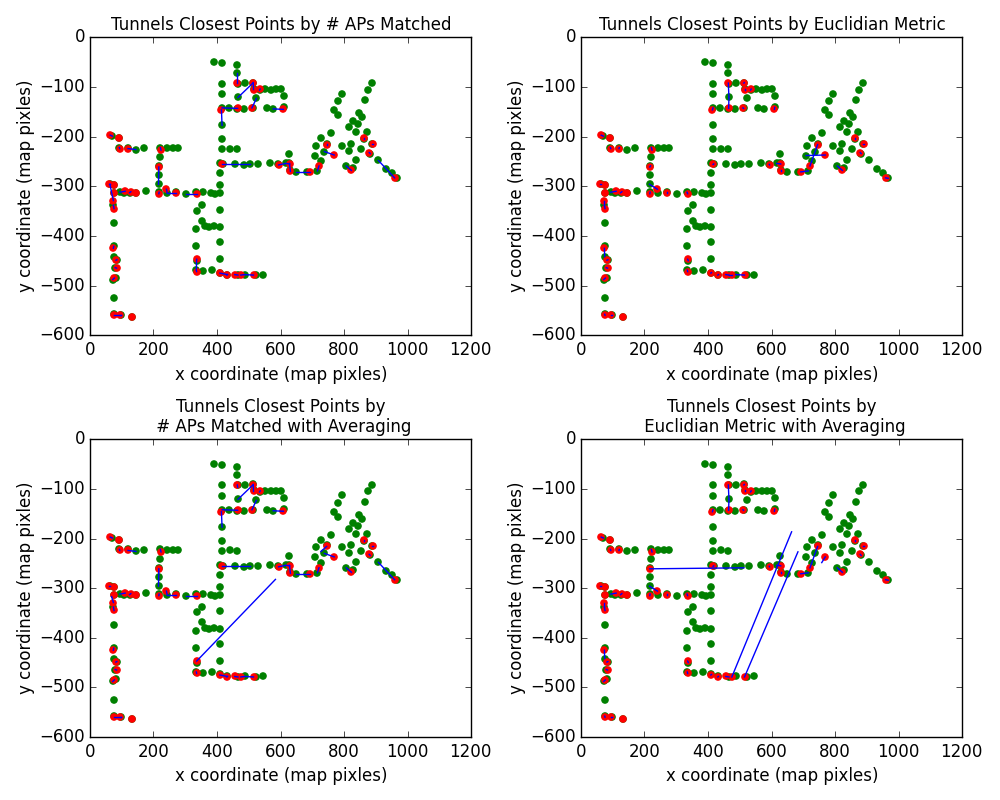
\includegraphics[width=0.9\textwidth]{tunnels_traintunnels_test_all_graphs.png}
\caption{Results through closest points in the tunnels using train-test data.}
\label{fig:tunnels_test}
\end{figure}

Note that for the above figure, most red points are connected to very close by green points, that’s why the lines are rather small. This can be observed better in the picture using zoom.
For the second set of experiments we wanted to test if doing indoor localization based on WiFi access points is actually more accurate, and could be used to localize at room level. This was another interesting question to explore since this is another instance when GPS signal would not be accurate enough. We collected data using two devices from one floor of Stata. Once again we used a train data and a test data. The plots can be found in the Appendix. We cross run the analysis by trying to predict the test data taken with one device by using the train data on the other device. These data did not perform too well. A key point is that one of our devices was relatively old and didn’t perform well even when we were using as both train and test data, the points acquired with that device. Overall, the main observation is that while our system is good enough to determine what side of the floor you’re in it doesn’t always correctly identify the room.
\section{Conclusion}
Localization using WiFi fingerprinting is a viable solution for some uses. In this report we applied the method to two scenarios. The first scenario was localization for the MIT tunnels, where the lack of signal makes GPS localization infeasible. For the second scenario we looked at the G5 floor of Stata and the aim was to determine in what office the user is currently located. While the method proved to be suited for the purpose of the first scenario it was not as efficient for the second one. Overall, the precision of Wifi fingerprinting alone seems severely limited, likely to a few meters; however, it is feasible to correctly identify the section of the building in which the user is located. It also has the advantage that no hardware beyond a wifi enabled device is needed. Given the current prevalence of smartphones, this is accessible to a large number of people. In addition, these solutions can be implemented purely in software and on the user side, making them easy to deploy. There are a number of algorithm avenues to explore which may improve the performance of a wifi fingerprinting based system and integrating other sensor data may allow one to further increase precision. In this paper we also described a number of challenges that will need to be addressed for this method of localization to be used in broader contexts; however, none of these problems seem insurmountable.
\section{Individual Contributions}
Each person on the team contributed roughly equally to the project. We all contributed to data collection. Everyone wrote one to two sections of the Final Report and we all revised it together.
Andrey was the main contributor to the application planning, designing and development. Madalina and Jayson were primarily responsible for the experiments, analysis and algorithm design.
\section{Acknowledgements}
We want to thank the 6.829 course staff, especially Dina Katabi, course instructor, and classes TAs Fadel and Omid of 6.829 Computer Networks for all the guidance throughout the semester.
% bibliography
\bibliographystyle{plain}
\bibliography{MITTunnelsBib}{}
\appendix
\section{Appendix: Further Analysis}
\begin{figure}[h]
\centering
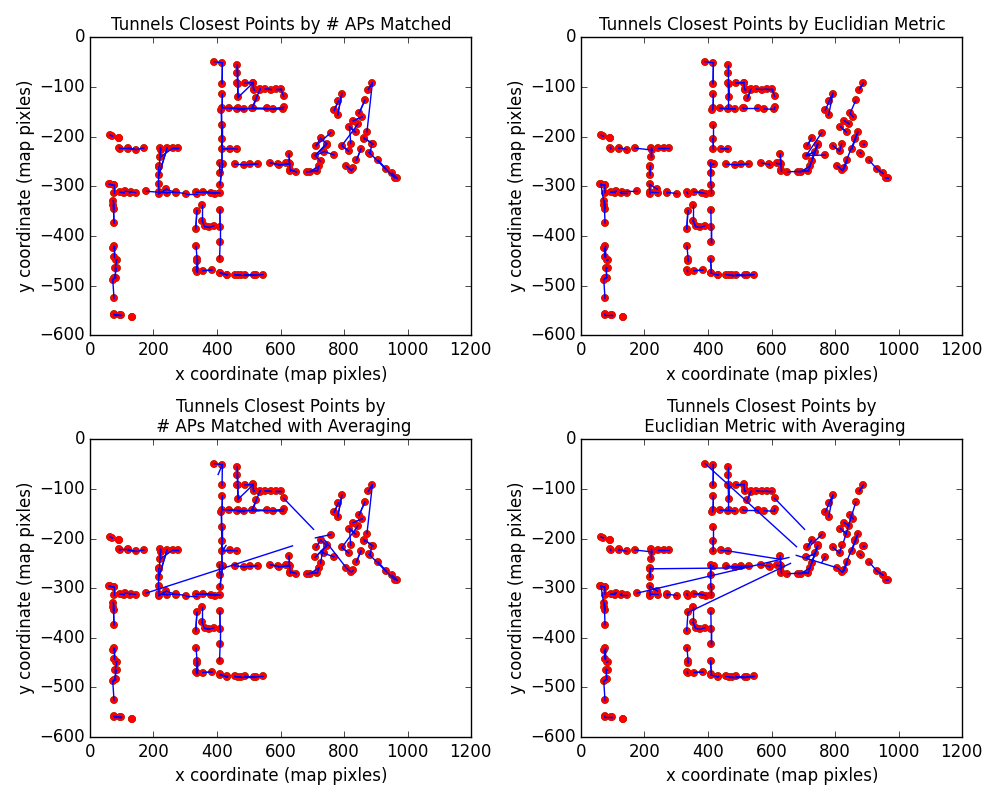
\includegraphics[width=0.9\textwidth]{tunnels_togethertunnels_together_all_graphs.png}
\caption{Results from calculating all pairs of closest points in the tunnels.}
\label{fig:tunnels_all}
\end{figure}
\begin{figure}[h]
\centering
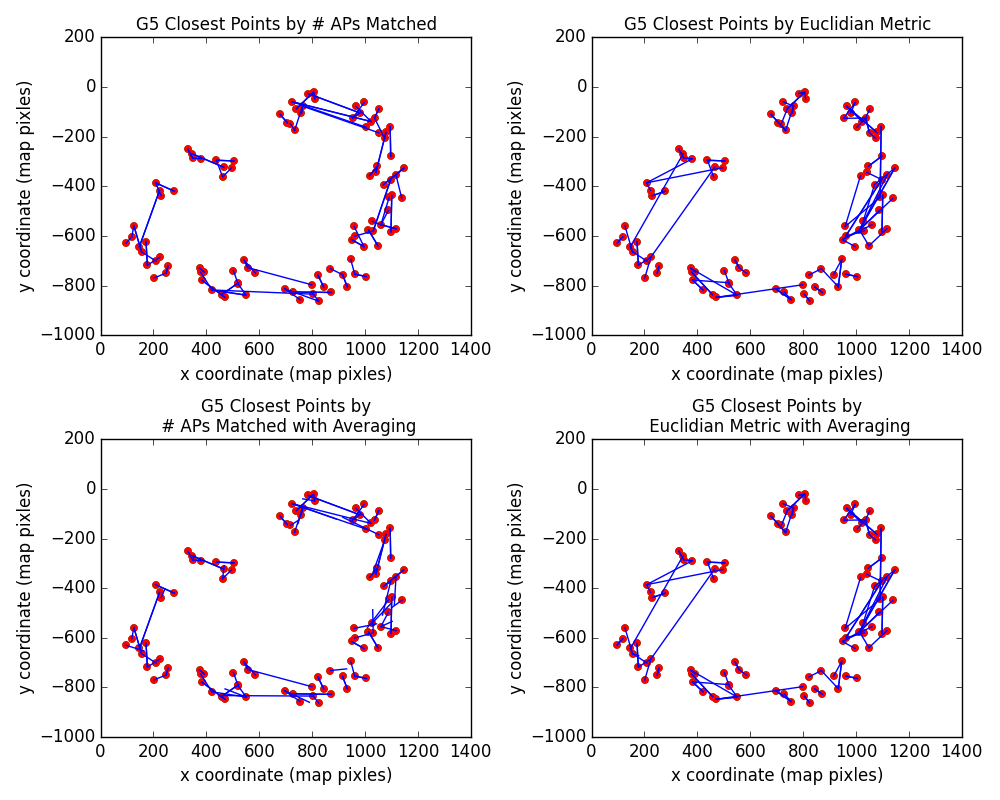
\includegraphics[width=0.9\textwidth]{nexusG5togethernexusG5together_all_graphs.png}
\caption{Results from calculating all pairs of closest points in G5 using data collected from the Nexus 5.}
\label{fig:tunnels_all}
\end{figure}
\begin{figure}[h]
\centering 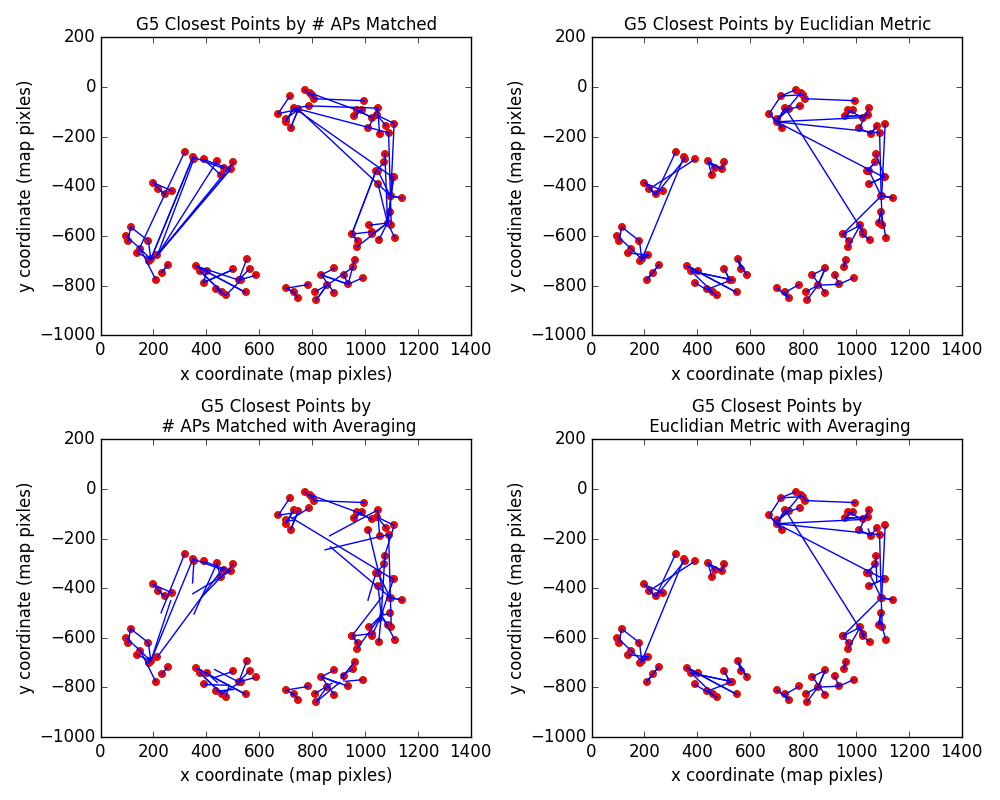
\includegraphics[width=0.9\textwidth]{samsungG5togethersamsungG5together_all_graphs.png}
\caption{Results from calculating all pairs of closest points in G5 using data collected from the Samsung Galaxy Tab 2.}
\label{fig:tunnels_all}
\end{figure}
\begin{figure}[h]
\centering 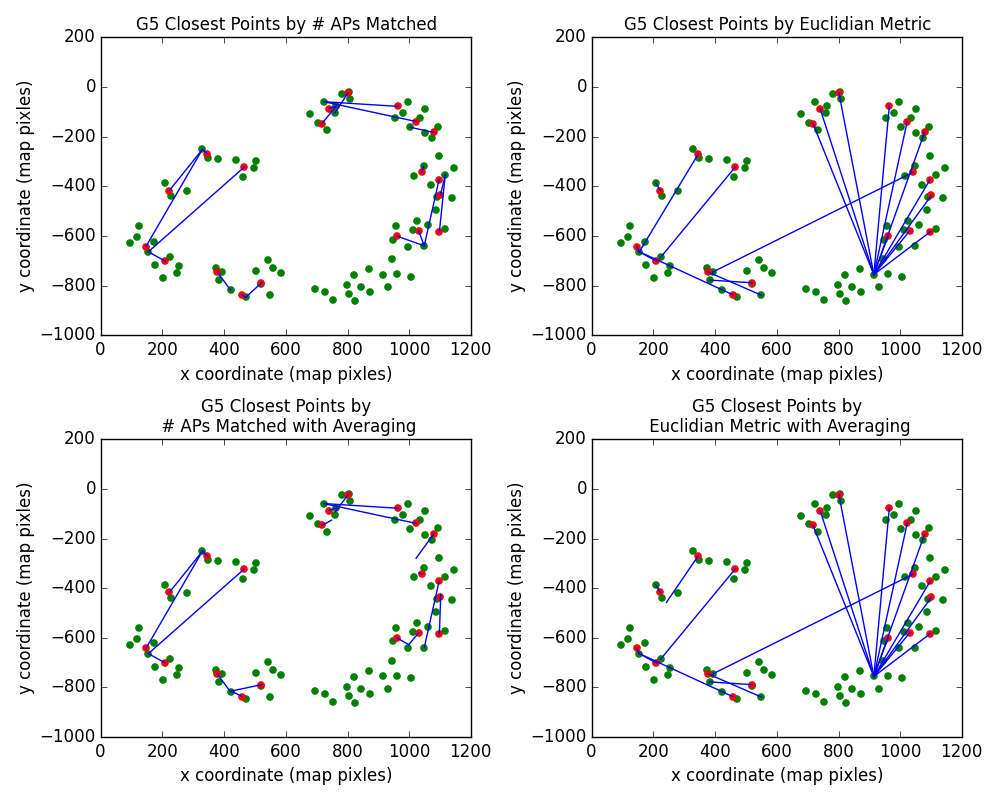
\includegraphics[width=0.9\textwidth]{nexusG5trainnexusG5test_all_graphs.png}
\caption{Results from the Nexus 5 test set on the Nexus 5 database for G5..}
\label{fig:tunnels_all}
\end{figure}
\begin{figure}[h]
\centering 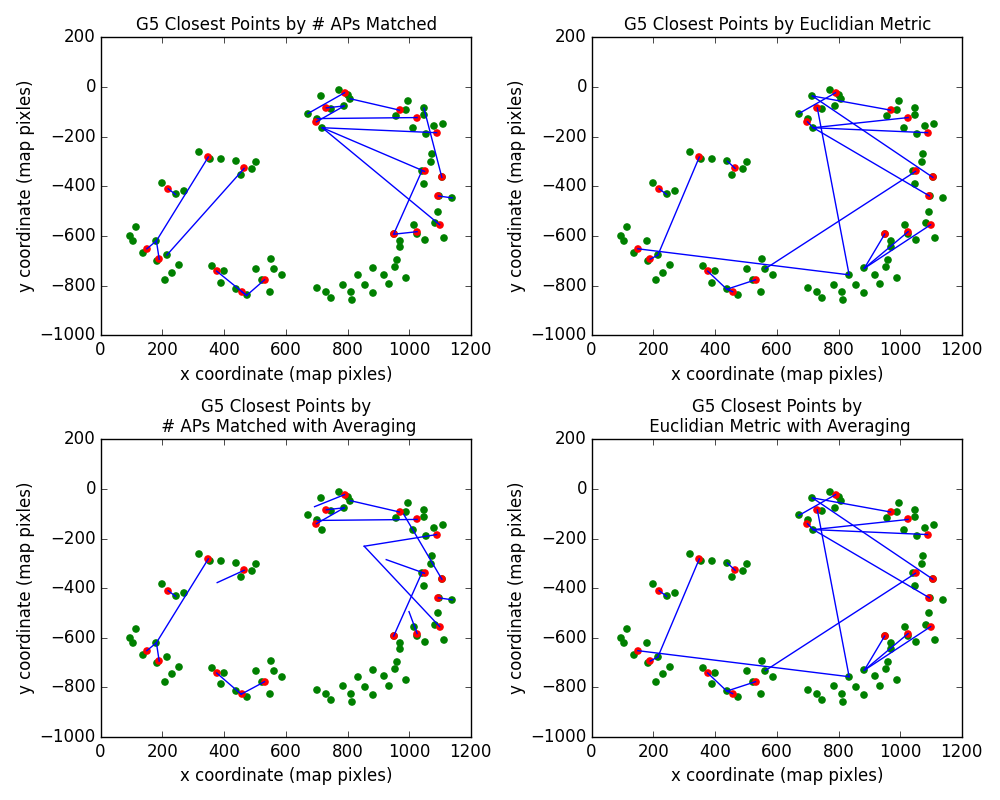
\includegraphics[width=0.9\textwidth]{samsungG5trainsamsungG5test_all_graphs.png}
\caption{Results from the Samsung Galaxy Tab 2 test set on the Samsung Galaxy Tab 2 database for G5..}
\label{fig:tunnels_all}
\end{figure}
\begin{figure}[h]
\centering 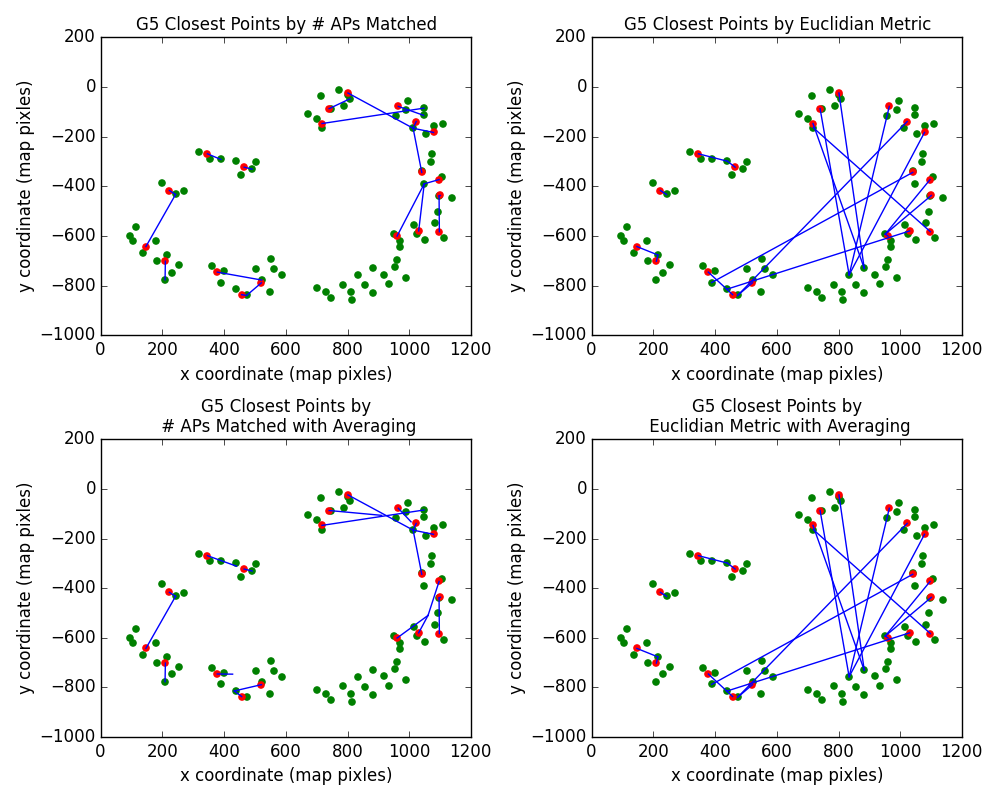
\includegraphics[width=0.9\textwidth]{samsungG5trainnexusG5test_all_graphs.png}
\caption{Results from the Samsung Galaxy Tab 2 test set on the Nexus 5 database for G5..}
\label{fig:tunnels_all}
\end{figure}
\begin{figure}[h]
\centering 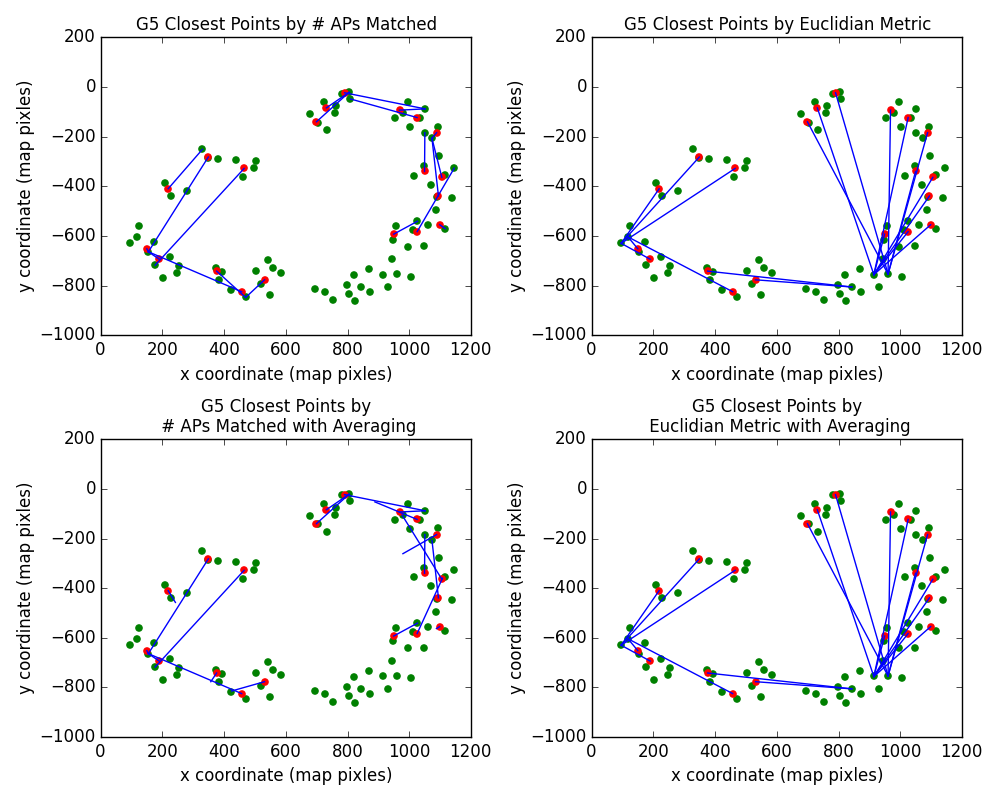
\includegraphics[width=0.9\textwidth]{nexusG5trainsamsungG5test_all_graphs.png}
\caption{Results from the Nexus 5 test set on the Samsung Galaxy Tab 2 database for G5..}
\label{fig:tunnels_all}
\end{figure}
\end{document}


